\documentclass[aspectratio=169, 11pt]{beamer}

% ---------------------------------------------------------
% Modern Theme: Metropolis + Fira Sans
% ---------------------------------------------------------
\usetheme[progressbar=frametitle, numbering=fraction, block=fill]{metropolis}
\usepackage[utf8]{inputenc}
\usepackage[T1]{fontenc}
\IfFileExists{FiraSans.sty}{\usepackage[sfdefault,light]{FiraSans}}{}
\usepackage{amsmath, amssymb}
\usepackage{graphicx}
\usepackage{booktabs}
\usepackage{tikz}
\usepackage[most]{tcolorbox}
\usepackage{hyperref}

% ---------------------------------------------------------
% Custom Modern Color Palette (Slate / Indigo / Cyan)
% ---------------------------------------------------------
\definecolor{SlateDark}{HTML}{0F172A}
\definecolor{SlateMed}{HTML}{1E293B}
\definecolor{AccentBlue}{HTML}{0284C7}
\definecolor{AccentIndigo}{HTML}{4F46E5}
\definecolor{AccentTeal}{HTML}{0D9488}
\definecolor{AccentAmber}{HTML}{D97706}
\definecolor{BgLight}{HTML}{F8FAFC}
\definecolor{CardBg}{HTML}{FFFFFF}
\definecolor{CardBorder}{HTML}{CBD5E1}

\setbeamercolor{normal text}{fg=SlateDark, bg=BgLight}
\setbeamercolor{frametitle}{fg=white, bg=SlateDark}
\setbeamercolor{progress bar}{fg=AccentBlue, bg=SlateMed}
\setbeamercolor{title separator}{fg=AccentBlue}
\setbeamercolor{alerted text}{fg=AccentIndigo}
\setbeamercolor{structure}{fg=AccentBlue}

% Adjust progress bar thickness
\makeatletter
\setlength{\metropolis@progressinheadfoot@linewidth}{2.2pt}
\setlength{\metropolis@titleseparator@linewidth}{2pt}
\makeatother

% Clean bullet styling
\setbeamertemplate{itemize item}{\textcolor{AccentBlue}{\large$\bullet$}}
\setbeamertemplate{itemize subitem}{\textcolor{AccentIndigo}{$\circ$}}

% Reusable modern card boxes
\newtcolorbox{icard}[2][AccentBlue]{
    enhanced,
    colback=CardBg,
    colframe=CardBorder,
    boxrule=0.6pt,
    borderline west={3.5pt}{0pt}{#1},
    arc=3pt,
    left=10pt, right=10pt, top=6pt, bottom=6pt,
    fonttitle=\bfseries,
    coltitle=SlateDark,
    attach title to upper={\\[4pt]},
    title={#2},
    halign=flush left
}

\newtcolorbox{plaincard}[1][AccentBlue]{
    enhanced,
    colback=CardBg,
    colframe=CardBorder,
    boxrule=0.6pt,
    borderline west={3.5pt}{0pt}{#1},
    arc=3pt,
    left=10pt, right=10pt, top=6pt, bottom=6pt,
    halign=flush left
}

% Presentation Metadata
\title{Parsa's Thesis}
\subtitle{First Meeting --- Ideas \& Research Overview}
\author{Parsa}
\date{\today}

\begin{document}

% ---------------------------------------------------------
% Slide 1: Title Slide (Dark Modern Style)
% ---------------------------------------------------------
{
\setbeamercolor{background canvas}{bg=SlateDark}
\setbeamercolor{normal text}{fg=white}
\usebeamercolor[fg]{normal text}
\begin{frame}[plain]
    \vspace{1.3cm}
    {\LARGE\textbf{Parsa's Thesis}\par}
    \vspace{0.25cm}
    {\large\textcolor{AccentBlue!45!white}{First Meeting --- Research Ideas \& Overview}\par}
    \vspace{0.35cm}
    \textcolor{AccentBlue}{\rule{0.32\textwidth}{2.2pt}}
    \vspace{0.7cm}

    {\normalsize\textbf{Parsa}\par}
    \vspace{0.15cm}
    {\small\textcolor{white!65!SlateDark}{\today}\par}
\end{frame}
}

% ---------------------------------------------------------
% Slide 2: Contents
% ---------------------------------------------------------
\begin{frame}{Contents}
    \begin{columns}[t, onlytextwidth]
        \begin{column}{0.48\textwidth}
            \begin{icard}[AccentBlue]{Research Roadmap}
                \begin{itemize}
                    \setlength\itemsep{0.35em}
                    \item \textbf{Project Seminar}
                    \item \textbf{RQs}
                    \begin{itemize}
                        \setlength\itemsep{0.2em}
                        \item RQ1 --- Prompt Injection \& Horizon
                        \item RQ2 --- Vector DB
                        \item RQ3 --- Rogue AI
                    \end{itemize}
                \end{itemize}
            \end{icard}
        \end{column}
        \begin{column}{0.48\textwidth}
            \begin{icard}[AccentIndigo]{Architecture \& Evaluation}
                \begin{itemize}
                    \setlength\itemsep{0.35em}
                    \item \textbf{BlackHole}
                    \item \textbf{Techs to use}
                    \item \textbf{Summary}
                    \item \textbf{Contact}
                \end{itemize}
            \end{icard}
        \end{column}
    \end{columns}
\end{frame}

% ---------------------------------------------------------
% Slide 3: RQ1 - Prompt Injection
% ---------------------------------------------------------
\begin{frame}{RQ1 --- Prompt Injection}
    \begin{plaincard}[AccentBlue]
        \textbf{Conformal Predictions}
    \end{plaincard}
    \vspace{0.2cm}
    \begin{plaincard}[AccentIndigo]
        \textbf{Certified Robustness}
    \end{plaincard}
    \vspace{0.2cm}
    \begin{plaincard}[AccentTeal]
        \textbf{Pearson inequality}
    \end{plaincard}
\end{frame}

% ---------------------------------------------------------
% Slide 4: RQ1 - Horizon (with Diagram)
% ---------------------------------------------------------
\begin{frame}{RQ1 --- Horizon}
    \begin{columns}[c, onlytextwidth]
        \begin{column}{0.30\textwidth}
            \begin{icard}[AccentBlue]{RQ1 --- Horizon}
                \small
                Only deterministic code makes security decisions; LLMs remain isolated behind strict labels and pointers.
            \end{icard}
        \end{column}
        \begin{column}{0.67\textwidth}
            \centering
            \begin{tcolorbox}[enhanced, colback=white, colframe=CardBorder, boxrule=0.6pt, arc=3pt, left=4pt, right=4pt, top=3pt, bottom=3pt, halign=center]
                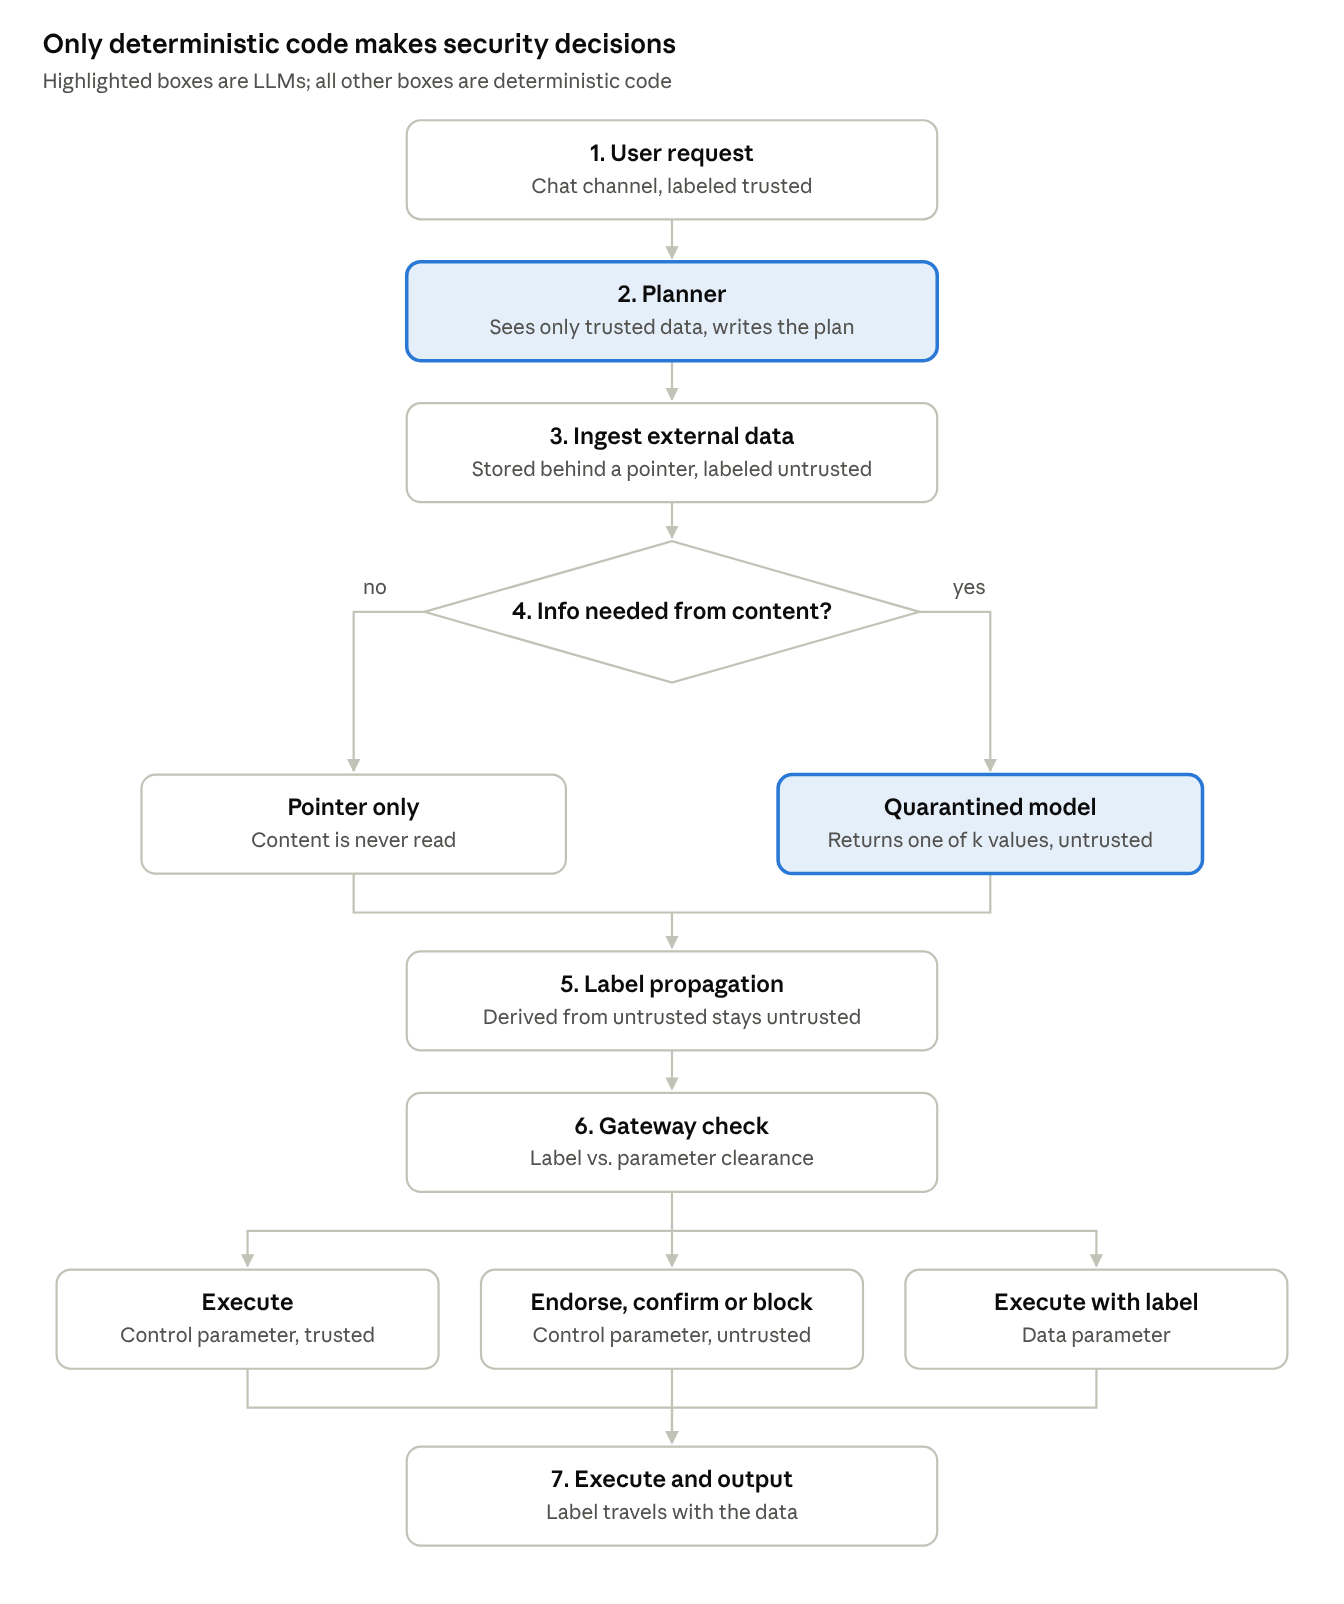
\includegraphics[height=0.73\textheight, keepaspectratio]{media/image1.png}
            \end{tcolorbox}
        \end{column}
    \end{columns}
\end{frame}

% ---------------------------------------------------------
% Slide 5: RQ2 - Vector DB
% ---------------------------------------------------------
\begin{frame}{RQ2 --- Vector DB}
    \begin{columns}[t, onlytextwidth]
        \begin{column}{0.48\textwidth}
            \begin{plaincard}[AccentBlue]
                \textbf{Differential Privacy}\\[2pt]
                \small To prevent Data Leakage
            \end{plaincard}
            \vspace{0.25cm}
            \begin{plaincard}[AccentIndigo]
                \textbf{DP-SGD concept}
            \end{plaincard}
        \end{column}
        \begin{column}{0.48\textwidth}
            \begin{plaincard}[AccentTeal]
                \textbf{Conformal Methods and bounds for poisoning}
            \end{plaincard}
            \vspace{0.25cm}
            \begin{plaincard}[AccentAmber]
                \textbf{GraphRAG relations poisoning}
            \end{plaincard}
        \end{column}
    \end{columns}
\end{frame}

% ---------------------------------------------------------
% Slide 6: RQ 3 - Rogue AI
% ---------------------------------------------------------
\begin{frame}{RQ 3 --- Rogue AI}
    \begin{icard}[AccentBlue]{Monitoring}
        \small
        \begin{itemize}
            \setlength\itemsep{0.35em}
            \item \textbf{Probability bounds for incoming malicious tokens:} This shall be over time, via Importance Sampling + extreme Power Law + Estimate Deployments scale
            \item \textbf{SPRT + E-values}
            \item \textbf{Ville's Inequality} (Vitllie Inequality)
            \item \textbf{Rare Event estimations}
        \end{itemize}
    \end{icard}
    \vspace{0.2cm}
    \begin{plaincard}[AccentIndigo]
        \textbf{Project Blackwall upgrade}
    \end{plaincard}
\end{frame}

% ---------------------------------------------------------
% Slide 7: BlackHole (with Image)
% ---------------------------------------------------------
\begin{frame}{BlackHole}
    \centering
    \begin{tcolorbox}[enhanced, colback=white, colframe=CardBorder, boxrule=0.6pt, arc=4pt, width=0.64\textwidth, halign=center, top=4pt, bottom=4pt]
        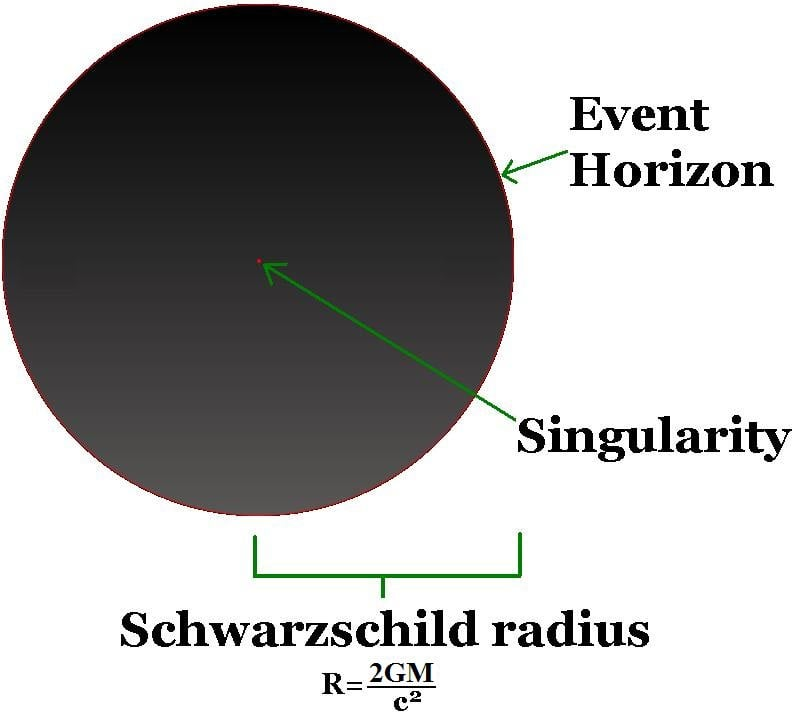
\includegraphics[height=0.69\textheight, keepaspectratio]{media/image2.jpeg}
    \end{tcolorbox}
\end{frame}

% ---------------------------------------------------------
% Slide 8: Worst Case Scenario on Each Step
% ---------------------------------------------------------
\begin{frame}{Worst Case Scenario on Each Step}
    \vspace{0.3cm}
    \begin{icard}[AccentIndigo]{Game-Theoretic Formulation}
        \Large\textbf{Sion Minimax Game}
    \end{icard}
\end{frame}

% ---------------------------------------------------------
% Slide 9: Evaluations
% ---------------------------------------------------------
\begin{frame}{Evaluations}
    \begin{plaincard}[AccentBlue]
        \textbf{DeepTeam}
    \end{plaincard}
    \vspace{0.2cm}
    \begin{plaincard}[AccentIndigo]
        \textbf{AgentDojo} (AgentDoji)
    \end{plaincard}
    \vspace{0.2cm}
    \begin{plaincard}[AccentTeal]
        \textbf{Hoeffding intervals}
    \end{plaincard}
\end{frame}

% ---------------------------------------------------------
% Slide 10: Summary
% ---------------------------------------------------------
\begin{frame}{Summary}
    \scriptsize
    \begin{columns}[t, onlytextwidth]
        \begin{column}{0.485\textwidth}
            \begin{plaincard}[AccentBlue]
                \begin{enumerate}
                    \setlength\itemsep{0.45em}
                    \item \textbf{Scope:} indirect (and direct) prompt injection in RAG/agent pipelines
                    \item \textbf{Spine:} IFC + noninterference with a proof, enforced by (a) \textbf{grammar-constrained decoding} that gives unauthorized tool calls zero probability, and (b) a \textbf{reference monitor that kills on violation} (Schneider: safety properties are enforceable)
                    \item \textbf{Probabilistic barriers:} perplexity filter, classifier, reasoning/task-alignment layer, \textbf{decoding-time suppression} (SafeDecoding/DExperts-style), optionally circuit breakers
                \end{enumerate}
            \end{plaincard}
        \end{column}
        \begin{column}{0.485\textwidth}
            \begin{plaincard}[AccentIndigo]
                \begin{enumerate}
                    \setcounter{enumi}{3}
                    \setlength\itemsep{0.35em}
                    \item \textbf{Internal signals $\rightarrow$ kill:} suppressed probability mass, entropy spike, attention shift (Attention Tracker)
                    \item \textbf{Game:} finite mixed-strategy minimax over barrier configs $\times$ attack classes; kills and false positives in the payoff
                    \item \textbf{Worst case:} game value capped by the IFC/monitor bound
                    \item \textbf{Evaluation:} DeepTeam + AgentDojo on open-weights models; attack success rate and utility, with Hoeffding interval
                    \item \textbf{Parking lot:} smarter thinking layer, edit automata
                \end{enumerate}
            \end{plaincard}
        \end{column}
    \end{columns}
\end{frame}

% ---------------------------------------------------------
% Slide 11: Techs to Use
% ---------------------------------------------------------
\begin{frame}{Techs to use}
    \scriptsize
    \begin{columns}[t, onlytextwidth]
        \begin{column}{0.48\textwidth}
            \begin{icard}[AccentTeal]{Nvidia}
                \begin{itemize}
                    \setlength\itemsep{0.15em}
                    \item Openshell
                    \item Model Optimizer
                    \item Garak
                    \item Guardrails
                \end{itemize}
            \end{icard}
            \vspace{0.15cm}
            \begin{icard}[AccentBlue]{Microsoft}
                \begin{itemize}
                    \setlength\itemsep{0.15em}
                    \item Spotlighting
                    \item GraphRAG
                \end{itemize}
            \end{icard}
        \end{column}
        \begin{column}{0.48\textwidth}
            \begin{icard}[AccentIndigo]{Google}
                \begin{itemize}
                    \setlength\itemsep{0.15em}
                    \item RRSI \& Dream-RSI
                    \item VeriHarness
                    \item CaMeL
                \end{itemize}
            \end{icard}
            \vspace{0.15cm}
            \begin{icard}[AccentAmber]{Tooling \& Open-Source}
                \begin{itemize}
                    \setlength\itemsep{0.15em}
                    \item Adversarial Robustness Toolbox (ART) v1.20
                    \item Unstract \& LLMWhisper
                    \item Chrootkit (Chtrootkit)
                    \item vLLM Guided Outline Decoding
                \end{itemize}
            \end{icard}
        \end{column}
    \end{columns}
\end{frame}

% ---------------------------------------------------------
% Slide 12: Contact
% ---------------------------------------------------------
{
\setbeamercolor{background canvas}{bg=SlateDark}
\setbeamercolor{normal text}{fg=white}
\usebeamercolor[fg]{normal text}
\begin{frame}[plain]
    \centering
    \vspace{1.6cm}
    {\LARGE\textbf{Contact}\par}
    \vspace{0.3cm}
    \textcolor{AccentBlue}{\rule{0.22\textwidth}{2.2pt}}
    \vspace{0.5cm}

    {\large Thank you!\par}
    \vspace{0.25cm}
    {\normalsize\textcolor{white!70!SlateDark}{Questions \& Discussion}\par}
\end{frame}
}

\end{document}
